\documentclass[conference]{IEEEtran}
\IEEEoverridecommandlockouts
% The preceding line is only needed to identify funding in the first footnote. If that is unneeded, please comment it out.
\usepackage{cite}
\usepackage{amsmath,amssymb,amsfonts}
\usepackage{algorithmic}
\usepackage{graphicx}
\usepackage{textcomp}
\usepackage{xtab}
\usepackage{xcolor}

\pagestyle{plain}
\pagenumbering{arabic}

\def\BibTeX{{\rm B\kern-.05em{\sc i\kern-.025em b}\kern-.08em
    T\kern-.1667em\lower.7ex\hbox{E}\kern-.125emX}}
    
\begin{document}

\title{HeartLink \\
    {\textsuperscript{}-An AI Family Platform for Rebuilding Connection-}
    }

\author{\IEEEauthorblockN{1\textsuperscript{st} Jeong Yeonkyung}
\IEEEauthorblockA{\textit{Dept. of Information Systems } \\
\textit{Hanyang Univ.}\\
Seoul, Republic of Korea \\
edaily0129@gmail.com}
\and
\IEEEauthorblockN{2\textsuperscript{nd} Kim Dayeon}
\IEEEauthorblockA{\textit{Dept. of Information Systems } \\
\textit{Hanyang Univ.}\\
Seoul, Republic of Korea \\
jewelry0706@hanyang.ac.kr}
\and
\IEEEauthorblockN{3\textsuperscript{rd} Park Jeongho}
\IEEEauthorblockA{\textit{Dept. of Information Systems } \\
\textit{Hanyang Univ.}\\
Seoul, Republic of Korea \\
popramel@hanyang.ac.kr}
\and
\IEEEauthorblockN{4\textsuperscript{th} Yu Jihye}
\IEEEauthorblockA{\textit{Dept. of Information Systems } \\
\textit{Hanyang Univ.}\\
Seoul, Republic of Korea \\
jihyeyu33@hanyang.ac.kr}
}

\maketitle

\begin{abstract}
In today's fast-paced world, staying connected with family and loved ones can be challenging, particularly for intergenerational families facing digital barriers. This project introduces a voice-based social networking service that transcends the limitations of text and photos, fostering natural and seamless daily sharing. Leveraging advanced AI technologies such as CLOVA voice recognition, OpenAI DALL-E 3 for image generation, and Google Cloud Vision for memory preservation, our platform allows users to share their lives through voice inputs that transform into dynamic text and image feeds. This approach supports natural communication, reduces the digital divide, and enhances family connections without requiring manual content creation.\\

The application's key features include a shared group feed for real-time updates, voice-to-text conversion, and AI-generated images based on textual input, enabling users to capture daily moments authentically. Additional functionalities like a family/friend photo album, AI collage, and a virtual pet "CLOi" to encourage family engagement further promote connectedness. With simple, voice-enabled interactions, users of all ages can effortlessly participate in family communication, making it a meaningful part of their daily routine.
\end{abstract}

\begin{IEEEkeywords}
Voice-based sharing, Family communication, AI-powered feed, Intergenerational connection, CLOVA voice recognition, DALL-E image generation, Memory preservation, Daily moments, Group photo album, Virtual pet CLOi
\end{IEEEkeywords}

\section{Role Assignment}
\begin{table}[htbp]
\begin{tabular}{|p{1cm}|p{1.7cm}|p{5cm}|}
    \hline
    Name & Roles & Task description and etc. \\
    \hline
    Jeong Yeonkyung & Development Manager, Software Developer (Back-end) & Oversees the development team, ensuring that the project is completed on time and within budget. Plans and implements the development methodology, sets team goals and deliverables, and provides mentoring and guidance to developers. Ensures code quality and adherence to standards. As a back-end developer, manages server-side infrastructure, optimizes databases, and handles SQL queries to ensure smooth operation of web and mobile applications. Technologies used include Python, Node.js, and JavaScript.\\
    \hline
        \end{tabular}
\end{table}
\begin{table}[htbp]
    \begin{tabular}{|p{1cm}|p{1.7cm}|p{5cm}|}
    \hline
    Kim Dayeon & Software Developer (Front-end), UI/UX Designer & As a front-end developer, leads the overall UI/UX page design of the software and personally carries out the development tasks. Ensures the user interface is not only visually appealing but also provides a seamless \\
    \hline
    \end{tabular}
\end{table}

\begin{table}[htbp]
\begin{tabular}{|p{1cm}|p{1.7cm}|p{5cm}|}
    \hline
    & & and intuitive user experience. Uses design tools like Figma to meticulously refine visual elements and user interactions. Implements the design using stylesheets such as Tailwind, ensuring a high level of interaction and functionality for users.\\
    \hline
\end{tabular}

 \begin{tabular}{|p{1cm}|p{1.7cm}|p{5cm}|}
    Park Jeongho & Software Developer (Front-end), User/Customer & As a front-end developer, designs and develops intuitive and efficient user interfaces based on user needs. Implements the interface using React-Native and JavaScript, ensuring easy navigation for users. Additionally, as a user/customer, contributes to making the service more accessible and usable for a wider audience.\\
    \hline
    Yu Jihye & Product Designer, Software Developer (AI) & Responsible for product design and integrating AI features. Develops AI models based on user data, ensuring the system adapts to users' needs. Utilizes AI to provide personalized recommendations and automates repetitive tasks, enhancing the overall user experience.\\
    \hline
\end{tabular}
\end{table}

\section{Introduction}
    \subsection{Motivation}
    Just Speak, and Stay Connected

    Communication remains essential to all relationships. However, as our lives grow increasingly busy, maintaining natural and effortless connections becomes ever more challenging. While we commonly share our daily lives through texts and photos, these methods can sometimes lose their authenticity. Now, there is a need for a new mode of connection—one that allows us to capture and share moments through voice.

    With advancements in voice recognition and AI technology, this vision has become achievable. Particularly in family communication, a system that records daily moments through voice and automatically generates a feed for sharing can profoundly enhance connections. By converting voice-recorded moments into text and images, and automatically delivering these to family members, this system allows for more seamless and genuine communication between parents and children, as well as across generations.

    For instance, parents can stay updated on their children's daily lives without needing direct contact, while children can remain connected with family members through shared voice and visual updates. This voice-based interface not only bridges the digital divide between generations but also fosters a more natural and continuous flow of family communication.

    \subsection{Problem Statements}
        \subsubsection{Difficulty in Naturally Sharing Daily Life}
        Current social media platforms primarily rely on text input and photo uploads, making it challenging for users to capture and share their daily lives naturally. In situations where hands are occupied or real-time sharing is desired, users often have to interrupt or modify their experiences to create content that fits platform requirements. This compromises the authenticity of moments shared and makes it difficult to convey emotional depth in these interactions.
        
        \subsubsection{Generational Gaps in Digital Accessibility}
        Existing social media interfaces do not adequately address the accessibility differences that arise from variations in age and digital proficiency, which poses limitations for intergenerational family communication. Elderly users often find complex text input methods and intricate menu structures challenging, while younger children may struggle to express themselves naturally within traditional interfaces. These generational gaps hinder regular family communication, creating the risk that the perspectives and experiences of certain family members may be excluded from the family's shared narrative.
        
        \subsubsection{Platform Limitations in Sustaining Family Connections}
        The structure of current platforms often hampers the long-term maintenance of family connections. The manual effort required for content creation and non-intuitive interfaces discourage ongoing engagement, particularly in family settings. For instance, children may find it burdensome to consistently share updates with parents, and parents may gradually lose touch with their children's daily lives. Furthermore, the lack of features for accumulating daily moments and emotions over time means that, as the years go by, these platforms fall short in supporting the depth and emotional bonds essential to lasting family relationships.

    \subsection{Solution}
        \subsubsection{Voice-Based Daily Sharing}
        Voice input alone enables natural daily sharing among family members. When speaking about daily experiences or thoughts, these vocal expressions automatically transform into text with relevant generated images, creating complete feeds. This direct voice-to-feed conversion eliminates manual text input or photo selection, making daily sharing effortless, especially during busy routines.

        \subsubsection{Family Connection Beyond Space and Time}
        Continuous family bonding transcends physical distance and lifestyle differences. Family members access shared moments at their convenience, removing time constraints from daily communication. Different time zones or busy schedules no longer hinder connection - each family member's daily life remains naturally shared and understood, maintaining meaningful relationships despite physical separation.

        \subsubsection{Cross-Generational Connection}
        Natural voice interaction eliminates digital barriers through simple conversation, without complex menus or text input. Elderly members unfamiliar with digital technology communicate easily through voice, while children express themselves freely through natural speech. This approach dissolves generational technology gaps, creating an inclusive environment where every family member participates naturally in daily sharing.

    \subsection{Research on Any Relative Software}
        \subsubsection{CLOVA Voice Recognition}
        Deep learning capabilities enable accurate voice capture even in multi-speaker environments. Real-time noise filtering captures natural home conversations while emotion analysis and context understanding detect subtle family nuances. Continuous learning adapts to each family's unique expressions and conversation patterns, delivering increasingly personalized and accurate recognition.

        \subsubsection{LG OpenAI DALL-E 3}
        Transforms daily moments into natural visual expressions. Creates high-quality images within two seconds based on voice or text input, adjusting styles to reflect conversational context and emotions. Generates safe, family-friendly images that richly express family moments and feelings while maintaining creative authenticity.

        \subsubsection{Google Cloud Vision}
        Securely preserves and organizes family memories with structured care. Ensures accurate facial recognition and scene analysis while prioritizing privacy protection, delivering quick responses through real-time processing. Meaningfully categorizes and arranges precious family moments, creating increasingly valuable memories over time.

\section{Requirement Analysis}
    \subsection{Common Features}
        \subsubsection{Sign-Up}
            Users can sign up to access all AI features such as voice-based daily sharing, AI-generated images, family/friend photo album, AI collage, virtual pet "CLOi", and cloud storage management. After signing up, access to additional features, such as personal data management and device linking, is determined based on user permissions.
            \begin{itemize}
                \item Enter phone number : The phone number is verified through an authentication system.
                \item Enter password : Passwords must be at least 8 characters long, with a mix of lowercase letters, numbers, and special characters.
                \item Enter name : The name is used as the user's default nickname on the platform.
            \end{itemize}

        \subsubsection{Log in}
            Users can access all AI features such as voice-based daily sharing, AI-generated images, family/friend photo album, AI collage, virtual pet "CLOi", and cloud storage management through a single log-in. After logging in, access to administrative functions like personal data and linked device management is determined by user permissions.

        \subsubsection{Find ID/Password}
            Users can retrieve their ID via email or phone number. If they forget their password, the platform provides a reset option through authentication via registered phone numbers or emails.

    \subsection{User-Specific Features}
        \subsubsection{Main Feed}
            The group feed is a space where users can see posts from themselves, family members, and friends. Through this feed, users can check real-time updates and share their daily moments effortlessly. Our app leverages AI functionality to help users easily create posts to share their lives. On the main screen, users can select a specific group, allowing posts to be visible only to that selected group.

            When creating a post, users can either compose it manually or choose from three AI-based post creation features:
            \begin{itemize}
                \item Voice Recognition-Based Text Creation: Users can dictate the content they want to include in a post, and AI will automatically convert it to text. This allows users to create posts without manually typing.
                \item Text-Based Image Generation: Based on the text written by the user or text created by AI based on users' voice input, AI generates an image. This allows users to include appropriate images in their posts without directly uploading photos, by generating images that match the written content.
            \end{itemize}

        \subsubsection{Post Archive}
            By tapping the 'Archive' button in the bottom navigation bar, users can access a personal archive where only their own posts are stored. Here, users can easily manage their posts, adjusting visibility settings (public/private), as well as editing or deleting specific posts.

        \subsubsection{Family/Friends Shared Photo Album}
            Users can create albums (folders) and select specific photos from their feed to include in these albums. By organizing photos into albums, users can manage which photos are displayed, and they can designate access permissions for each album, allowing only family members or close friends to view them.

            \begin{itemize}
                \item AI Collage Creation: Based on the photos in the shared photo album, AI can generate a "memory collage." This collage visually captures memories and gives a decorative effect. With a simple "Create" button, users can generate this collage, and the resulting collage can be downloaded for individual storage.
            \end{itemize}

        \subsubsection{Adding Friends}
            Although this SNS primarily focuses on family interaction, users can also add friends to share photos with them. This feature is designed for users who want to communicate with friends as well as family members.

        \subsubsection{Raising Our Family's Pet CLOi}
            To motivate family participation in the SNS, we introduced a feature to raise a virtual pet called "CLOi." Similar to the "Sumone" app, this pet character grows based on the frequency of posts and photo uploads. It encourages group members to participate actively and promotes family bonding.

\section{Development Environment}
    \subsection{Choice of Software Development Platform}
        \subsubsection{Estimated Cost}
            \begin{itemize}
                \item AWS EC2 \& S3: About 3 USD per month
            \end{itemize}
        
        \subsubsection{Development Platform : Windows}
            Windows serves as our primary development platform, providing comprehensive support for React Native and Node.js development environments. It offers seamless integration with essential development tools and frameworks, enhancing overall development productivity. Windows' user-friendly interface simplifies environment configuration and project management, while its robust community support ensures quick problem resolution. The platform's continuous updates and improvements guarantee access to the latest development technologies, making it an ideal choice for our cross-platform mobile application development.

        \subsubsection{Programming Languages : JavaScript}
            JavaScript stands as our core programming language, offering versatility for both frontend and backend development. Its extensive ecosystem and wide community support provide numerous libraries and tools essential for modern web development. JavaScript's interpreted nature enables rapid development and easy debugging, while its asynchronous capabilities make it particularly suitable for building responsive applications. The language's ubiquity ensures excellent documentation and resource availability, significantly enhancing development efficiency.

        \subsubsection{Frameworks \& Database}
            \begin{itemize}
                \item React Native: React Native emerges as our primary framework for mobile application development. This JavaScript-based framework enables the development of native mobile applications for both iOS and Android platforms. React Native's component-based architecture promotes code reusability and maintainable structure, while its hot reloading feature accelerates the development process by enabling immediate code change verification. The framework's bridge to native components ensures high performance and authentic native user experiences, making it an optimal choice for our mobile application development.

                \item Express.js: Express.js functions as our backend framework, providing a minimalist yet robust solution for building web applications and APIs. Built on Node.js, it offers excellent performance for handling asynchronous operations and real-time data processing. The framework's middleware system allows for flexible request handling and modular application structure. Express.js's seamless integration with MongoDB through Mongoose enables efficient database operations, while its extensive ecosystem of middleware packages enhances development capabilities.

                \item MongoDB: MongoDB serves as our primary database system, offering a flexible and scalable NoSQL solution for our application's data management needs. Through Mongoose ODM (Object Data Modeling), it provides a structured way to model application data and enforce data schemas while maintaining MongoDB's dynamic nature. MongoDB's document-oriented structure aligns perfectly with JavaScript's JSON format, making it naturally compatible with our Node.js/Express.js backend. The database's powerful querying capabilities, along with its ability to handle large volumes of unstructured data, make it ideal for social media applications that require efficient storage and retrieval of various content types including user profiles, posts, and media metadata. Its scalability and performance in handling concurrent operations make it particularly suitable for real-time applications with frequent data updates and complex data relationships. 
            \end{itemize}

            \subsection{Software in Use}
        \begin{figure}[htbp]
            \centerline{
\includegraphics[width=3cm, height=3cm]{Images/logo/vsc.png}}
            \caption{Logo of Visual Studio Code}
            \label{fig}
        \end{figure}
        \subsubsection{Visual Studio Code (VS Code)}
            Visual Studio Code, commonly known as VS Code, is a lightweight yet powerful code editor developed by Microsoft. It supports various programming languages and provides essential tools like syntax highlighting, debugging, and integrated Git support. VS Code is highly extensible, allowing developers to customize the editor through a vast library of extensions to suit their specific needs. The editor's user-friendly interface and frequent updates contribute to its popularity among developers. Its ability to handle large codebases and quick access to useful extensions make it ideal for both web and mobile development.

        \begin{figure}[htbp]
            \centerline{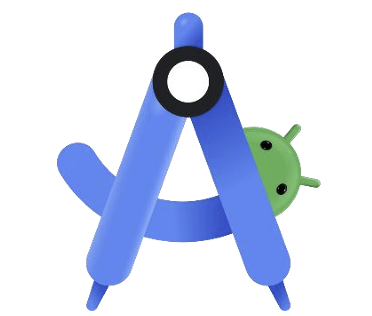
\includegraphics[width=3cm, height=3cm]{Images/logo/android.png}}
            \caption{Logo of Android Studio}
            \label{fig}
        \end{figure}
        \subsubsection{Android Studio}
            Android Studio serves as the primary integrated development environment (IDE) for Android application development. It provides comprehensive tools essential for React Native development, including the Android SDK manager, device emulators, and debugging capabilities. The platform's advanced emulator system allows developers to test applications across various Android versions and device configurations, ensuring broad compatibility. Android Studio's performance profiling tools help optimize application performance, while its integrated debugging features enable efficient problem resolution. With built-in support for version control systems and continuous integration, Android Studio streamlines the development workflow for mobile applications.

        \begin{figure}[htbp]
            \centerline{
\includegraphics[width=3cm, height=3cm]{Images/logo/expo.png}}
            \caption{Logo of Expo}
            \label{fig}
        \end{figure}
        \subsubsection{Expo}
            Expo is a framework and a platform for universal React applications, enabling developers to build, deploy, and maintain React Native applications more easily. It provides a set of tools and services, including a development client, pre-built libraries, and an online publishing platform, that streamline the app development process. With Expo, developers can preview changes instantly on physical devices without complex configurations. Expo also supports the integration of native modules, making it easier to access device-specific features. Its simplicity and support for hot reloading make Expo a popular choice for building cross-platform mobile apps.

        \begin{figure}[htbp]
            \centerline{
\includegraphics[width=4cm, height=3cm]{Images/logo/zustand.png}}
            \caption{Logo of Zustand}
            \label{fig}
        \end{figure}
        \subsubsection{Zustand}
            Zustand is a lightweight state management library for React applications. It provides a simple API for managing global state, allowing developers to avoid prop drilling by sharing state across components directly. Zustand's minimal setup and component-based approach make it easy to use and integrate into existing projects. The library supports both synchronous and asynchronous state updates, giving developers flexibility in handling complex state logic. Its simplicity and efficiency make Zustand an ideal choice for managing application state in a straightforward and maintainable way.

        \begin{figure}[htbp]
            \centerline{
\includegraphics[width=5cm, height=2cm]{Images/logo/figma.png}}
            \caption{Logo of Figma}
            \label{fig}
        \end{figure}
        \subsubsection{Figma}
            Figma is a collaborative design tool widely used for creating user interfaces, prototypes, and interactive design elements. Its web-based nature allows teams to work together in real-time, making it ideal for cross-functional collaboration between designers and developers. Figma supports a variety of design elements and offers tools for creating responsive designs, making it a versatile choice for UI/UX design. Developers can easily inspect design specs, export assets, and view design changes live, enhancing communication and workflow efficiency. With its user-friendly interface and cloud-based functionality, Figma has become a popular choice for modern design teams.

        \begin{figure}[htbp]
            \centerline{
\includegraphics[width=4cm, height=4cm]{Images/logo/aws.png}}
            \caption{Logo of Amazon EC2}
            \label{fig}
        \end{figure}
        \subsubsection{Amazon EC2}
            Amazon EC2 (Elastic Compute Cloud) is a part of Amazon Web Services (AWS) that provides scalable virtual servers in the cloud. Developers can configure and launch EC2 instances to run various applications, giving them control over the underlying computing resources. EC2 supports a wide range of instance types optimized for different workloads, including CPU-intensive and memory-intensive tasks. It is ideal for deploying web applications, backend services, and data processing workloads, as it allows for flexible scaling to meet demand. With robust security options and integration with other AWS services, EC2 is widely used in cloud-based infrastructures.

        \begin{figure}[htbp]
            \centerline{
\includegraphics[width=4cm, height=3cm]{Images/logo/awss3.png}}
            \caption{Logo of Amazon S3}
            \label{fig}
        \end{figure}
        \subsubsection{Amazon S3}
            Amazon S3 (Simple Storage Service) is a highly scalable cloud storage service provided by AWS, designed to store and retrieve any amount of data. It allows developers to create and manage buckets for organizing data, which can be used for hosting static websites, archiving, and data backups. S3's durability and high availability make it suitable for critical data storage, while its integration with other AWS services enhances data management flexibility. S3 also supports versioning and access controls, allowing for secure data storage and retrieval. This service is essential for applications requiring reliable and scalable storage solutions.

        \begin{figure}[htbp]
            \centerline{
\includegraphics[width=6cm, height=2cm]{Images/logo/compass.png}}
            \caption{Logo of MongoDB Compass}
            \label{fig}
        \end{figure}
        \subsubsection{MongoDB Compass}
            MongoDB Compass serves as our primary database management tool, providing a graphical user interface for interacting with MongoDB databases. It offers intuitive features for data visualization, query building, and schema analysis, making database operations more accessible and efficient. The tool's ability to perform CRUD operations visually, along with its real-time data insights and performance monitoring capabilities, greatly enhances database management and debugging processes. MongoDB Compass's schema visualization and query optimization suggestions help developers maintain efficient database operations and optimize application performance.

        \begin{figure}[htbp]
            \centerline{
\includegraphics[width=6cm, height=2cm]{Images/logo/postman.png}}
            \caption{Logo of Postman}
            \label{fig}
        \end{figure}
        \subsubsection{Postman}
            Postman functions as our API development and testing platform, enabling comprehensive testing and documentation of our REST APIs. It provides a user-friendly interface for creating, organizing, and executing HTTP requests, making API testing and debugging more efficient. The tool's ability to create test suites, set up automated testing environments, and generate API documentation streamlines the API development process. Postman's collaboration features allow team members to share collections and environments, ensuring consistency in API testing across the development team. Its request history and response validation features make it invaluable for API debugging and optimization.
            
        \begin{figure}[htbp]
            \centerline{
\includegraphics[width=4cm, height=4cm]{Images/logo/firebase.png}}
            \caption{Logo of Firebase}
            \label{fig}
        \end{figure}
        \subsubsection{Firebase}
            Firebase serves as our comprehensive backend service provider, particularly focusing on user authentication, push notifications, and real-time data synchronization. Its authentication system supports multiple sign-in methods including email/password, social media integration, and phone number verification, ensuring secure and flexible user access. The Firebase Cloud Messaging (FCM) system enables efficient delivery of push notifications to mobile devices, enhancing user engagement. Its real-time database capabilities and cloud functions provide scalable infrastructure for handling real-time features and background tasks. Firebase's integration with Android and iOS platforms makes it an ideal choice for building cross-platform mobile applications with robust backend services.

        \begin{figure}[htbp]
            \centerline{
\includegraphics[width=5cm, height=2cm]{Images/logo/whisper.png}}
            \caption{Logo of Whisper}
            \label{fig}
        \end{figure}
        \subsubsection{Whisper}
            Whisper is a general-purpose speech recognition model developed by OpenAI, trained on 680,000 hours of multilingual speech data. It is released as open-source software that anyone can freely use, and provides various features centered on STT (Speech-to-Text) functionality that converts speech into text. The key features include speech recognition, language identification, translation, and subtitle generation, with support for 99 different languages. It offers broad applicability as it can recognize dialects and accents of major languages including Korean, English, Chinese, and Japanese. The Whisper v2-large model is currently available through OpenAI's free API under the model name whisper-1.

        \begin{figure}[htbp]
            \centerline{
\includegraphics[width=7cm, height=2.5cm]{Images/logo/kospeech.png}}
            \caption{Logo of KoSpeech}
            \label{fig}
        \end{figure}
        \subsubsection{KoSpeech}
            Kospeech is an open-source toolkit that provides Korean speech recognition models, released by developer Kim Soohwan in 2020. The models in Kospeech follow an End-to-End approach, where End-to-End refers to a method that allows the model to learn all features contained in speech data, including grammar and pronunciation. A distinctive characteristic of this approach is that it takes raw audio as a complete input. The process works by taking audio signals as input, extracting features, and then passing these features through the model and CTC algorithm to produce text output. To implement STT (Speech-to-Text), Kospeech utilizes AI hub's Kspon dataset, which consists of 1,000 hours of Korean speech data along with its transcribed labels. The toolkit provides three different preprocessing methods for this data. Built on the PyTorch framework, Kospeech specifically focuses on Korean language support and offers various models and frameworks including DeepSpeech2, LAS (Listen, Attend and Spell), and SpeechTransformer.

        \begin{figure}[htbp]
            \centerline{
\includegraphics[width=6cm, height=1.5cm]{Images/logo/dalle.png}}
            \caption{Logo of DALL·E}
            \label{fig}
        \end{figure}
        \subsubsection{DALL·E}
            DALL·E is an AI image generation system developed by OpenAI that can create realistic images and artwork based on natural language descriptions. Released in November 2023, the latest version, DALL·E 3, is notable for its integration with ChatGPT. Having been trained on diverse captions and images created through OpenAI's specially designed captioning tools, it can accurately understand user prompts and generate highly consistent and aesthetically pleasing images. Currently, DALL·E 3 offers the ability to create new images of specific sizes based on prompts. The previous version, DALL·E 2, was released in November 2022 and supports the ability to edit existing images or create variations of user-provided images. Currently, both DALL·E 3 and DALL·E 2 are available through OpenAI's Images API, and ChatGPT Plus subscribers can directly experience DALL·E 3's image generation capabilities through ChatGPT.

        \begin{figure}[htbp]
            \centerline{
\includegraphics[width=6cm, height=2cm]{Images/logo/aihub.png}}
            \caption{Logo of AI-Hub}
            \label{fig}
        \end{figure}
        \subsubsection{AI-Hub}
            AI-Hub is an integrated platform that provides comprehensive support for AI infrastructure needed for AI technology, product, and service development. It is designed to allow anyone to utilize and participate in AI technology by providing AI data, AI SW APIs, and computing resources. The platform specifically offers AI training data across 14 different fields and publishes AI training datasets held by various domestic and international institutions and companies. AI-Hub provides an open API called 'aihubshell' that enables easy downloading of artificial intelligence training data. It enhances developer accessibility by supporting a data downloader that can be used in various development environments, including Linux.

        \begin{figure}[htbp]
            \centerline{
\includegraphics[width=6cm, height=3cm]{Images/logo/github.png}}
            \caption{Logo of GitHub}
            \label{fig}
        \end{figure}
        \subsubsection{GitHub}
            GitHub is an essential platform for version control and collaboration in software development. It provides a centralized repository for code, allowing multiple developers to work on the same project simultaneously and manage changes efficiently. Through features like pull requests, issue tracking, and branching, GitHub enables teams to review code, track project progress, and manage tasks effectively. It also integrates with numerous development tools, facilitating seamless workflows. With an active community and extensive documentation, GitHub supports both open-source and private projects, making it a versatile tool for developers.

        \begin{figure}[htbp]
            \centerline{
\includegraphics[width=5cm, height=3cm]{Images/logo/redmine.png}}
            \caption{Logo of Redmine}
            \label{fig}
        \end{figure}
        \subsubsection{Redmine}
            Redmine functions as our project management tool, offering comprehensive features for tracking tasks, issues, and project milestones. Its robust ticketing system enables detailed task assignment and progress monitoring, while the built-in time tracking capabilities help in managing project timelines effectively. Redmine's customizable workflow and permission systems allow for precise control over project processes and access rights. The platform's Gantt charts and calendar views provide clear visualization of project timelines and deadlines, making it an essential tool for maintaining project organization and team accountability.

        \begin{figure}[htbp]
            \centerline{
\includegraphics[width=6cm, height=2cm]{Images/logo/notion.png}}
            \caption{Logo of Notion}
            \label{fig}
        \end{figure}
        \subsubsection{Notion}
            Notion is an all-in-one workspace that combines note-taking, project management, and knowledge sharing in one platform. Its flexible, block-based structure allows users to organize content in various formats, including text, tables, images, and databases, making it suitable for diverse tasks. Notion supports real-time collaboration, enabling team members to work on shared documents and tasks seamlessly. It is commonly used for creating wikis, project boards, and personal notes, as it provides extensive customization options. With its intuitive interface and robust features, Notion is a valuable tool for organizing and managing project information.

        \begin{figure}[htbp]
            \centerline{
\includegraphics[width=6cm, height=2cm]{Images/logo/slack.png}}
            \caption{Logo of Slack}
            \label{fig}
        \end{figure}
        \subsubsection{Slack}
            Slack serves as our primary team communication platform, facilitating real-time collaboration and information sharing among team members. It provides organized communication through dedicated channels for different topics and projects, along with direct messaging capabilities for private conversations. Slack's robust integration capabilities with development tools like GitHub and various AWS services enable automated notifications and streamlined workflows. The platform's searchable history and file-sharing features make it invaluable for maintaining team documentation and quick information retrieval. Its mobile and desktop applications ensure team members stay connected and responsive regardless of their location.

        \begin{figure}[htbp]
            \centerline{
\includegraphics[width=5cm, height=2cm]{Images/logo/overleaf.png}}
            \caption{Logo of Overleaf}
            \label{fig}
        \end{figure}
        \subsubsection{Overleaf}
            Overleaf is an online collaborative platform specifically designed for LaTeX document creation, popular among researchers, students, and academics. It provides a real-time LaTeX editor, allowing users to collaborate on complex documents containing mathematical equations, tables, and references. Overleaf simplifies the writing process by offering a LaTeX compiler with instant previews, enabling authors to see how their documents look as they type. The platform also supports version control and can integrate with GitHub, making it easy to manage large projects with multiple contributors. Overleaf’s cloud-based nature makes it accessible from any device, enhancing the document creation process for scientific writing.
            
\section{Requirement Specifications}
    \subsection{Loading Page}
        When an application communicates with servers, a delay is inevitable in the process. During the delay, it might show just a blank screen to users. To prevent users from getting a blank page, a loading screen will appear instead. This applies to all functions that require server communication.

        This loading page UI is made by 'skeleton' from React Native. While receiving data from the server, components without received data shows that it is loading. In other words, while server is processing and receiving data after a http request has been made by the client. It can make a seamless and user friendly UI by using the loading screen. 
        
\subsection{Log-in Page}
        The login page serves as the initial entry point of the application. Without a login, it is impossible to use any of the functions of the app. If the application is not logged in, users can create their own account or login using an account they have created before.

        In a back-end point of view, The client collects the user's phone number and password and sends a request to Firebase Authentication when the login button is pressed. Firebase handles the authentication process and returns a JWT token. The token has an expiration time for security purposes and needs to be refreshed periodically. After Firebase authentication succeeds, the application server (running on Amazon EC2) receives the user information and handles the session management. Express.js backend stores essential user data in MongoDB and manages user sessions.

        In a front-end point of view, when a user taps on either the phone number or password input field in the React Native application, the field's border becomes highlighted with the application's brand color, and the mobile keyboard appears. The screen automatically adjusts upward when the keyboard appears to ensure input fields remain visible. If the user enters their phone number and presses the next button on the keyboard, the focus automatically moves to the password field. The password is masked with dots while being entered for security. Both phone number and password fields must contain valid input for the login button to become active. When the login button is pressed, it enters a loading state while the authentication process occurs. After successful login, the user is directed to the main feed view of the social networking application. If the login fails, an alert message appears explaining the error, and the user remains on the login screen to try again.

    \subsection{Register Page}
        For the registration process, users must provide their phone number which serves as their unique identifier in the system. The registration flow begins with phone number verification through Firebase Authentication. Users enter their phone number and receive a verification code via SMS. Once verified, they proceed to fill in additional required information including name, nickname (displayed to other users in the SNS platform), password, and password confirmation.

        On the client side, built with React Native and managed with Zustand for state management, there are immediate validations for input format and matching password fields. The UI follows the application's design system created in Figma, maintaining consistency with the login screen's behavior. The registration button activates only when all fields are properly filled and validated.

        When submitted, the verified user data is first processed through Firebase Authentication, and upon success, the additional user information is sent to our Express.js backend running on EC2. The backend performs secondary validation before storing the user profile in MongoDB, with any user-uploaded profile images being stored in Amazon S3. If registration succeeds, users are redirected to the login page. In case of failure, appropriate error messages are displayed through the app's alert system, allowing users to correct their input and try again.

    \subsection{Dashboard (Main Feed Page)}
        The dashboard page is the main feed page (main page) that is first shown to users after login succeeds. The main function of the dashboard page is showing all of the friends' real-time latest posts. To help this objective, users can infinitely scroll down the page. Also the user can delete or revise the post through the delete/revise button on the top-right side of the post.

        These two buttons are basically invisible, but only the post owner can see them. And the emotion emojis below the post content are the emotions for the users can select his/her own daily mood. The only selected emotion is shown as opacity 100\% and the others are as transparency 50\%. These data can be sourced from the MongoDB database and the AWS S3 cloud then shown to the users.

        At the bottom of the screen, there is a menu bar that can lead user to another screen and functions. For the main menu bar, there are AI-CLOI, AI-album, main feed, friend list, and my page. At the top of the screen, if the user presses the middle '—' button, the screen is transited to the group selection screen.

        It's a screen composed of tabs, and from the user's perspective, it's not ideal to send requests every time you switch tabs, as it can cause delays. Therefore, as soon as user enters this screen, all the data is fetched all at once. This data is stored in a context for later use.

    \subsection{Add-Friends Page}
        To share the posts with other users, a user should add other users as 'friend'. The friend means they can make a group and can see their posts each other. If a user presses the 'friend' tab in the main menu bar, the friend list screen is shown and the user can search for the users through the add (+) button in the right-bottom side of the screen.

        Users can search for other users by his/her nickname. Then after user1 adds user2 as friend, the friend request message is sent to the user2. User2 can see this message through the notification function. If the user2 accepts, they be 'friend' from that time. In the friend list, if the user presses the trash can icon button, the user can delete the selected user from friend list.

    \subsection{Add-Groups Page}
        In the group list screen, if user can presses group for a long time, the user can change group name, and if he/she just tab once, the group member list is shown. If the user want to delete a member, then he/she can do this through trash can icon. If the user want to delete the group, he/she should delete all of the members.

        If a user presses the '—' button at the top of the main feed page, all of the group list page is shown to users. If the user presses the trash icon button in the friend list, the selected user is deleted from the friend list. The add (+) button in the right-bottom side is group creation button. If a user presses it, the group name input pop up is shown and the user can make a new group. The group name must be up to 6 Korean letters and the "Group name must be up to 6 letters." error message is shown in pop up if the size is over 6 letters. Successfully making group name, the screen is transited to friend list screen, and the user can add friends to the group or change group to another.

    \subsection{Album Page - AI-Collage}
        [-------------------------------------------------]

    \subsection{Feed Upload Page - AI Voice Recognition}
        In the feed upload process of the application, users are presented with voice recognition functionality powered by OpenAI API for converting spoken words into text. When accessing the feed upload screen, users can tap the microphone button to activate the voice recognition interface, which displays a visual audio waveform animation during recording.

        The recorded voice is processed through the OpenAI API for real-time speech-to-text conversion. The interface also provides an alternative option where users can bypass the voice recognition feature and directly input text using the keyboard, offering flexibility in content creation. The text input field features a clean, minimalist design that follows the application's visual style guide created in Figma.

        As users speak or type, the text appears in real-time, and they can edit or modify it before proceeding to the next step of adding visual content to their post.

    \subsection{Feed Upload Page - AI Image Creation}
        After obtaining the text content, either through voice recognition or manual input, the feed creation process moves to the visual content stage. Here, users are presented with two options: AI image generation or manual image selection from their gallery.

        When users choose AI image generation, the application processes the input text through an AI image generation model to create a visual representation of the text content. The generated image appears on the screen, displayed in a format optimized for the social media feed. If users are not satisfied with the initially generated image, they can tap the regenerate button to create a different variation based on the same text input.

        Alternatively, users have the option to select images directly from their device's gallery instead of using the AI-generated images. The gallery selection interface allows users to choose multiple images from their local storage. Whether using AI-generated images or manually selected ones, all visual content is stored in Amazon S3 cloud storage, while the post metadata and references are managed in MongoDB through the Express.js backend running on Amazon EC2. The entire upload process is managed through React Native's state management using Zustand, ensuring a smooth and responsive user experience throughout the content creation flow.

    \subsection{AI-CLOI Page}
        The application features an AI companion called CLOI, which grows and evolves based on user engagement and activity within the platform. CLOI starts as a baby (LV.1) and progressively grows through stages - infant (LV.2), child (LV.3), teenager (LV.4), and adult (LV.5) - as users create and share more content on the platform.

        Each evolution level of CLOI is visually represented by different facial expressions and characteristics that reflect its growth stage, creating an emotional connection with users. The evolution system is managed through the Express.js backend, which tracks the number of posts created by the user and stores the progress in MongoDB.

        When users reach certain posting milestones, CLOI automatically evolves to its next stage, with the transition animated to celebrate the growth moment. CLOI also functions as an interactive AI companion that generates personalized greetings and friendly messages for users. Using the OpenAI API, CLOI analyzes the user's activity patterns, posting frequency, and time of day to create contextually appropriate and engaging messages.

        For example, CLOI might say "I see you're working hard on creating content today!" or "It's been a while since your last post, would you like to share something new?" These interactions are designed to encourage user engagement while maintaining a friendly, supportive presence. The message generation system considers CLOI's current evolution level, ensuring that the tone and complexity of interactions match its growth stage, making the experience more authentic and emotionally resonant. The entire CLOI system is integrated into the React Native frontend using Zustand for state management, ensuring smooth animations and transitions between different states and messages.

    \subsection{Notification Page}
        The notification system in the application keeps users informed about interactions with their content and friend activity through Firebase Cloud Messaging (FCM). When a new notification arrives, a red dot indicator appears on the notification bell icon in the top right corner of the main page, providing a visual cue for unread notifications.

        These notifications can be viewed in two ways: as push notifications delivered through FCM when the app is in the background, or as in-app alerts that slide down from the top of the screen for active users. The notification page displays a chronological history of all notifications, with each entry showing the interacting user's profile picture, the specific action taken, and relevant timestamps.

        For friend requests, users can respond directly through accept or decline buttons on the notification entry. The notification data is managed through the Express.js backend and stored in MongoDB, while the frontend uses React Native with Zustand for state management, ensuring smooth rendering and real-time updates of notification status.

    \subsection{My Page}
        The My Page serves as a personal archive space where users can manage their profile and access their content history. At the top of the page, users can view and edit their profile information, including their nickname which can be modified by tapping on it.

        The page displays key statistics about the user's activity, including the total number of posts created and their current CLOI companion level. A "10-day posting streak" badge with a fire emoji indicates active user engagement, encouraging consistent platform participation.

        The page features two main archival sections: "My Posts" and "My Album". The My Posts section provides access to a chronological feed of all text-based and AI-generated content the user has shared on the platform. The My Album section serves as a dedicated photo gallery, organizing all images the user has uploaded through their posts, whether they were AI-generated or manually uploaded from their device.

        All content data is stored in Amazon S3 with references maintained in MongoDB, while the frontend interface is built using React Native with Zustand managing the state for smooth navigation and content loading. The layout follows the application's consistent design language, providing an intuitive and organized way for users to revisit and manage their content history.

\end{document}
